%%%%%%%%%%%%%%%%%%%%%%%%%%%%%%%%%%%%%%%%%
% Conference Booklet
% LaTeX Template
% Version 1.0 (22/12/2019)
%
% This template originates from:
% https://www.LaTeXTemplates.com
%
% Authors:
% Maxime Lucas (ml.maximelucas@gmail.com) 
% Pau Clusella
% Modifications for LaTeX Templates by Vel (vel@LaTeXTemplates.com)
%
% License:
% GNU General Public License v3.0
%
%%%%%%%%%%%%%%%%%%%%%%%%%%%%%%%%%%%%%%%%%

%----------------------------------------------------------------------------------------
%	PACKAGES AND OTHER DOCUMENT CONFIGURATIONS
%----------------------------------------------------------------------------------------

\documentclass[
	openany, % Allow chapters to start on odd and even pages
	parskip=false, % Large space between paragraphs
	12pt, % Default font size
	a4paper, % Paper size, use letterpaper for US letter size
]{conferencebooklet} % Custom class defining the style and layout of the template

%----------------------------------------------------------------------------------------
\usepackage[doipre={DOI:~}]{uri}
\usepackage{textcomp}


\begin{document}

%----------------------------------------------------------------------------------------
%	 COVER PAGE
%----------------------------------------------------------------------------------------

%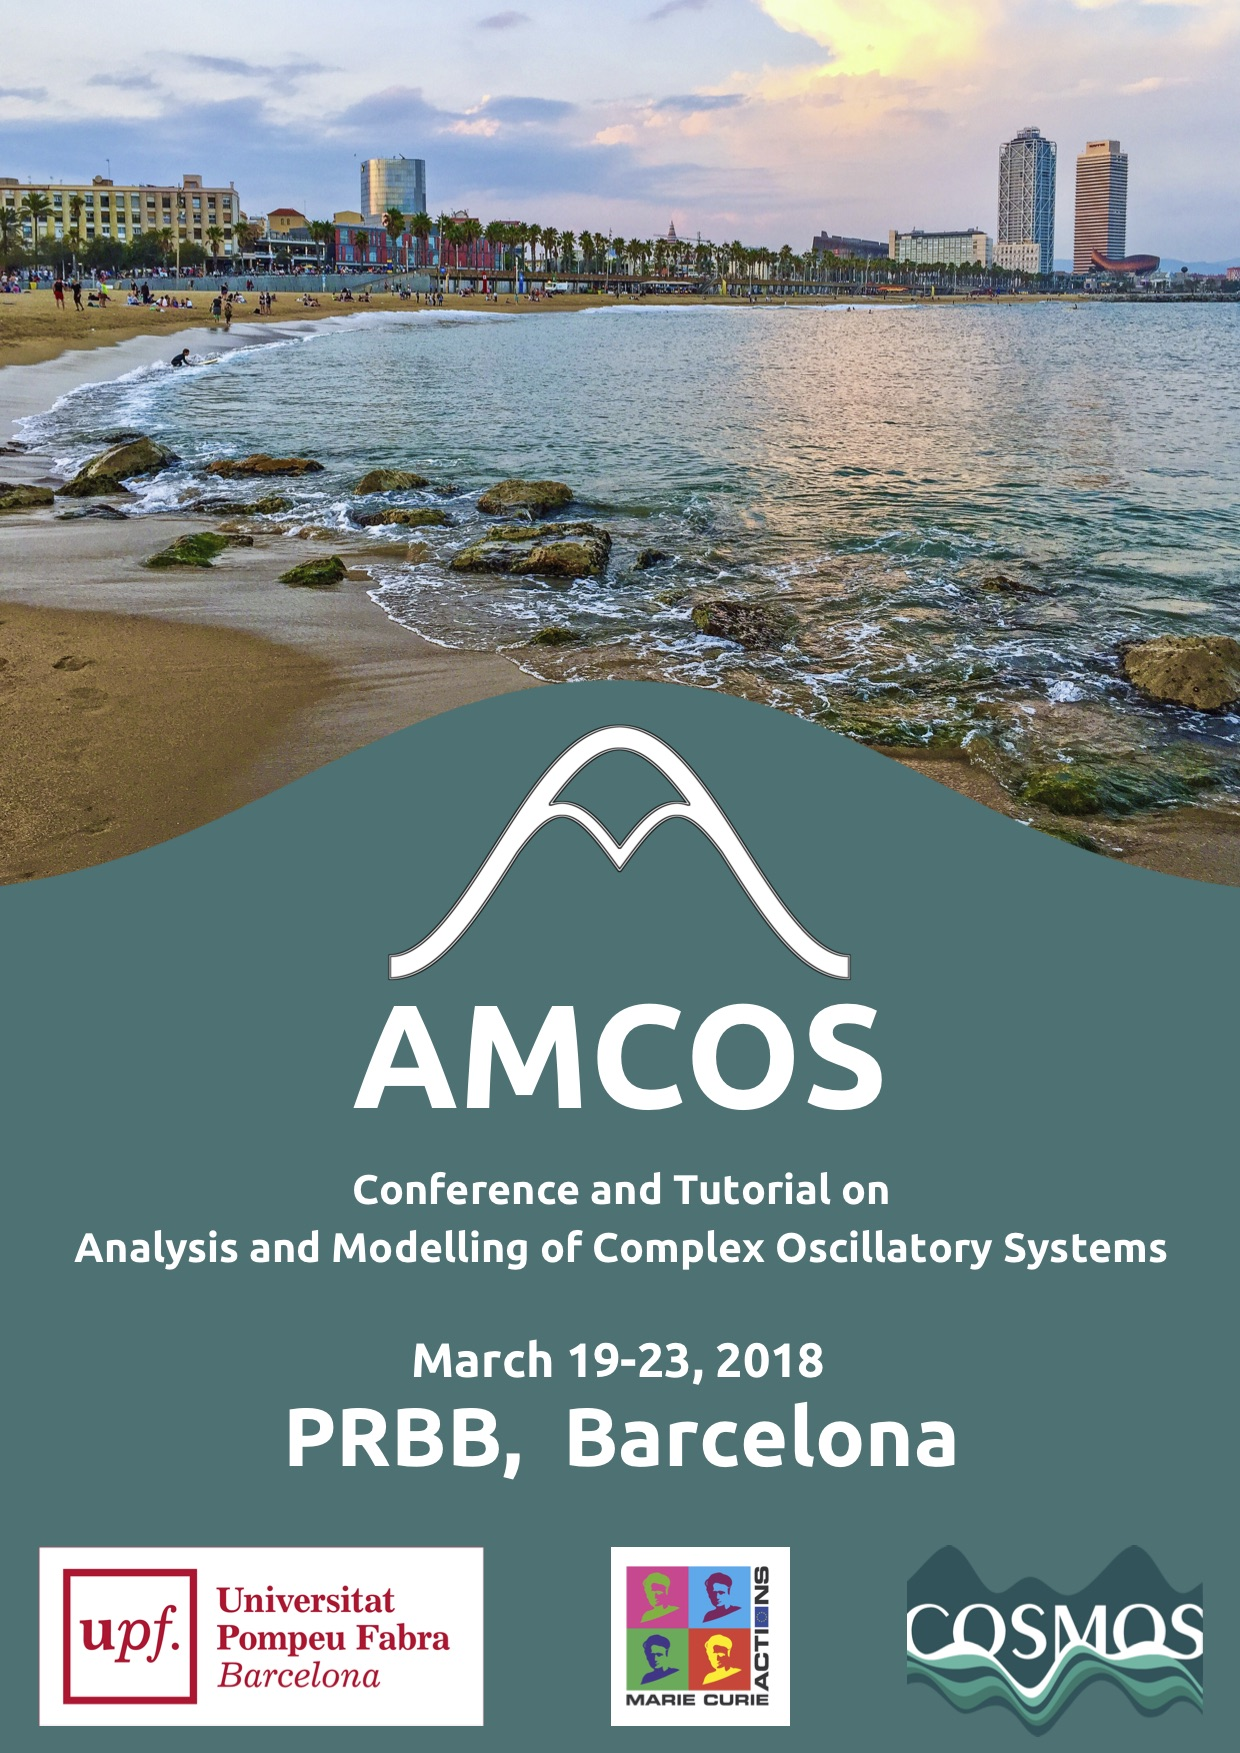
\includepdf{images/cover.jpg} % The cover for the booklet is included as a whole-page image, it can be a PDF or an image file but must be the same dimensions as the paper size

%----------------------------------------------------------------------------------------
%	 INFORMATION/COPYRIGHT PAGE
%----------------------------------------------------------------------------------------

\thispagestyle{empty} % Suppress headers and footers on this page

~\vfill % Push text down
% TODO: \usepackage{graphicx} required


\begin{center}	
Geomorfologický sborník 20\\
\vspace{2em}
Sborník abstraktů\\
\vspace{2em}
State of geomorphological research in 2022\\
\vspace{2em}
Book of Abstracts\\
May 18 – 20, 2022 in Horní Bečva (Czech Republic)\\
\vspace{2em}
Editors: Michal Břežný\\ \vspace{2em}
The contributions contained in this publication have not been edited by language and 
typographic appeal. The authors are responsible for the linguistic and content quality of texts.
\\ \vspace{2em}

Publisher: University of Ostrava, Ostrava \\\vspace{2em}

© 2022 Michal Břežný\\
\vspace{2em}
ISBN xxxxxxxxx\\

\vspace{5em}




%	This is the short version of the booklet for print use. \\ Full abstracts with all authors, references, and figures can be found at:\\ \url{https://amcosconference.com/}

	This booklet is created using \LaTeX{} template which is based on the original version at:\\ \url{https://github.com/maximelucas/AMCOS\_booklet}
\end{center}
\begin{figure}[t]
	\centering
	
\includegraphics[width=1\linewidth]{images/geomorfologie-logolink}
	
\end{figure}
\newpage

%----------------------------------------------------------------------------------------
%	 TABLE OF CONTENTS
%----------------------------------------------------------------------------------------

\tableofcontents

%----------------------------------------------------------------------------------------
%	 ABOUT CONFERENCE
%----------------------------------------------------------------------------------------

\chapter{About}
\section{State of geomorphological research in 2022}
\noindent
Forthcoming event is organised bilaterally and should be perceived as the common conference of both Czech Association of Geomorphologists and Association of Slovak Geomorphologists. Considering the 2-year pause due to the world pandemics, it will be a round anniversary (20\textsuperscript{th} in the line of meetings started in 2000) for the Czech Association of Geomorphologists, and it will also be the 11\textsuperscript{th} biennial meeting for the Association of Slovak Geomorphologists.

The thematic scope of the conference traditionally covers all geomorphological disciplines as well as those of related geosciences. The conference will culminate with a whole-day field trip. We hope the conference will be interesting and inspiring and we are looking forward for your valuable contributions.

\section{Organizing committee}

\begin{center}
	\begin{tabular}{l l l}
		RNDr. Veronika Kapustová, Ph.D. & Ing. Anna Kidová, PhD. & prof. RNDr. Tomáš Pánek, Ph.D.\\
		Mgr. Radek Tichavský, Ph.D. & RNDr. Jan Lenart, Ph.D. & doc. RNDr. Tomáš Galia, Ph.D.\\
		RNDr. Václav Škarpich, Ph.D. & Mgr. Michal Břežný, Ph.D. & doc. RNDr. Jan Hradecký, Ph.D.\\
		prof. RNDr. Karel Šilhán, Ph.D. &Mgr. Ján Novotný, PhD. & Mgr. Miloš Rusnák, PhD.\\
		Mgr. Zuzana Połedniková & Mgr. Adriana Holušová & Mgr. Vladimír Chalupa\\
		Mgr. Lukáš Vaverka & Mgr. Andrea Fabiánová & Mgr. Andrius Toločka 
	
	\end{tabular}
\end{center}

% TODO: \usepackage{graphicx} required
\begin{figure}
	\centering
	\includegraphics[width=0.9\linewidth]{"images/logos/Partnerlogos/2022 04 25 záštita ČGS geomorfologové 1"}
	\label{fig:2022-04-25-zastita-cgs-geomorfologove-1}
\end{figure}


%----------------------------------------------------------------------------------------
%	 TIMETABLE
%----------------------------------------------------------------------------------------

\chapter{Timetable}

\section{Preconference workshop}

\begin{longtable}{|C{0.15\linewidth}| C{0.04\linewidth}|  C{0.3\linewidth} C{0.0\linewidth} C{0.4\linewidth}|}\hline	
	\eventtype{}{Tuesday May 17, 2022}
	\tablebreak{12:00--13:00}{Arrival/accommodation of the participants}
	\tablebreak{13:00--17:00}{Field survey and data acquisition on the Bečva River}
	\tablebreak{17:00--19:00}{Data processing}
	\eventtype{}{Wednesday May 18, 2022}
	\tablebreak{9:00--12:00}{Data processing and modelling, presentation of the results}

\end{longtable}

\section{Wednesday May 18, 2022}
\begin{longtable}{|C{0.15\linewidth}| C{0.04\linewidth}|  C{0.3\linewidth} C{0.0\linewidth} C{0.4\linewidth}|}\hline	
	\tablebreak{9:00--13:00}{Registration}
	\tablebreak{13:00}{Conference opening, invited lectures}
	\tablebreak{15:30}{Oral presentations}
	\tablebreak{17:00}{Poster session}
	\tablebreak{19:00}{Plenary meeting of the Czech Association of Geomorphologists}
	\tablebreak{19:00}{Plenary meeting of the Association of Slovak Geomorphologists}
\end{longtable}

\section{Wednesday May 18, 2022}
\begin{longtable}{|C{0.15\linewidth}| C{0.04\linewidth}|  C{0.3\linewidth} C{0.0\linewidth} C{0.4\linewidth}|}\hline	
	\tablebreak{8:30--17:00}{Oral presentations}
	\tablebreak{17:00}{Poster session}
	\tablebreak{20:00}{Closing ceremony, Festive dinner}
\end{longtable}

\newpage

%------------------------------------------------
%
%\section{Wednesday, 21 of March}
%
%\begin{longtable}{|C{0.15\linewidth}| C{0.04\linewidth}|  C{0.3\linewidth} C{0.0\linewidth} C{0.4\linewidth}|}\hline	
%	\IS{9:00-9:40}{Hiroya Sato}{Tokyo, Japan}{Title of invited speaker}
%	\CT{9:40-10:10}{Marc Fournier}{Brussels, Belgium}{Title of contributed talk}
%	\IS{10:10--12:45}{Hiroya Sato}{Tokyo, Japan}{Title of invited speaker}
%	\tablebreak{10:45--11:10}{Coffee}
%	%odor
%	\CT{11:10--11:40}{Marc Jansen}{Amsterdam, The Netherlands}{Title of contributed talk and references and a figure}
%	\CT{11:40--12:10}{Marc Jansen}{Amsterdam, The Netherlands}{Title of contributed talk and references and a figure}
%	\IS{12:10--12:45}{Hiroya Sato}{Tokyo, Japan}{Title of invited speaker}
%	\tablebreak{12:45--14:00}{Lunch}
%	\CT{14:00--14:30}{Marc Fournier}{Brussels, Belgium}{Title of contributed talk}
%	\CT{14:30-15:00}{Marc Fournier}{Brussels, Belgium}{Title of contributed talk}
%	\eventtype{16:30--18:00}{Excursion}
%	\eventtype{20:00}{Conference Dinner}
%\end{longtable}

%------------------------------------------------

\section{Thursday, 22 of March}

%\begin{longtable}{|C{0.15\linewidth}| C{0.04\linewidth}|  C{0.3\linewidth} C{0.0\linewidth} C{0.4\linewidth}|}\hline	
%	\IS{9:00 -- 9:40}{Hiroya Sato}{Tokyo, Japan}{Title of invited speaker}
%	\IS{9:40--10:20}{Hiroya Sato}{Tokyo, Japan}{Title of invited speaker}
%	\IT{10:20--10:45}{Franck Schmidt}{Munich, Germany}{A special talk about diversity in science}
%	\tablebreak{10:45--11:10}{Coffee}
%	\CT{11:10-11:40}{Marc Jansen}{Amsterdam, The Netherlands}{Title of contributed talk and references and a figure}
%	\KL{11:40--12:35}{Leon Tremblay}{Montreal, Canada}{Title of a keynote lecture}
%	\eventtype{12:35--12:45}{Poster Prize \& Conclusion}
%	\tablebreak{12:45--14:00}{Lunch}
%\end{longtable}

%----------------------------------------------------------------------------------------
%	 LIST OF TALK ABSTRACTS
%----------------------------------------------------------------------------------------

% Abstract template
%\abstract
%	{} % Title
%	{} % Author(s)
%	{} % Tag, can be: empty, \KLtag (keynote lecture), \IStag (invited speaker), \CTtag (contributed talk) or \ITtag (invited talk)
%	{} % Affiliation(s)
%	{} % Abstract text

\chapter{List of Abstracts}


%start of abstract
%\abstract
%{} % Title
%{} %short author -- toc
%{\textsuperscript{1}*} % Author(s)
%{\KLtag} % Tag, can be: empty, \KLtag (keynote lecture), \IStag (invited speaker), \CTtag (contributed talk) or \ITtag (invited talk)
%{
%	\textsuperscript{1}
%	\textsuperscript{2}
%	\textsuperscript{3}
%}
%} % Affiliation(s)
%{}  %e-mail
%{}%keywords
%{
%}%abstract
%{
%}%references
%end of abstract

%%%%%%%%%%%%%%%%%%%%%%%%%%%%%%%%%%%%%%%%%%%%%%%%%%%%%%%%%%%%%%%%%%%%%%%%%%%%%%%%%%%%%%%%%%%%%%
%start of abstract
\abstract
{Dendrogeomorphic Dating in the Ostrava-Karviná Mining Landscape: Processes, Events, Responses} % Title
{Tichavský et al.} %short author -- toc
{Radek Tichavský\textsuperscript{1}*, Andrea Fabiánová\textsuperscript{1}, Eva Jiránková\textsuperscript{2}, Jan Lenart\textsuperscript{1}, Lucie Polášková\textsuperscript{1}, \\Radim Tolasz\textsuperscript{3}
} % Author(s)
{\TLtag} % Tag, can be: empty, \KLtag (keynote lecture), \IStag (invited speaker), \CTtag (contributed talk) or \ITtag (invited talk)
{
\textsuperscript{1}Department of Physical Geography and Geoecology, Faculty of Science, University of Ostrava, Chittussiho 10, 710 00 Ostrava, Slezská Ostrava, Czech Republic\\
\textsuperscript{2}Institute of Geonics of the Czech Academy of Sciences, Studentská 1768, 708 00 Ostrava, Czech Republic\\
\textsuperscript{3}Czech Hydrometeorological Institute, Na Šabatce 17, 143 06 Praha 4, Czech Republic
} % Affiliation(s)
{radek.tichavsky@osu.cz}  %e-mail
{mining landscape, dendrogeomorphology, subsidence, landslide, compression wood, Ostrava-Karviná mining district}%keywords
{Mining-induced subsidence is a worldwide environmental problem that leads to damage to infrastructure and property; thus, knowledge of its past–recent development is critically needed during land-use planning. We dated the activity of gravitational processes related to mining-induced subsidence using dendrogeomorphic methods at four sites in the Upper Silesian Coal Basin near the former mines of the Karviná mining district. The landslide/subsidence sites were characterised by scarps, rotated blocks, stepped relief with grabens, pressure folds, and shallow movements within landslide toes or within flat undulating relief. Based on 644 increment cores from 161 trees, we were able to identify subsidence/landslide activity, with the most frequent responses occurring from the late 1950s to the early 1970s and from 2005 to 2011. The highest number of tree ring records dates back to 1973. Moreover, more than 30\% of tilted trees from the landslide sites created compression wood at multiple directions indicated complex deformations. At the other sites, the occasional occurrence of single rings with isolated compression wood was included as a possible indicator of events due to frequent coincidence with common series of compression wood. A comparison of tree-ring-based chronology with in situ monitoring revealed good synchronicity with the periods of increased subsidence rates (between 1 and 3 m.year\textsuperscript{−1}). In addition, not only mining operations, but also the occurrence of extreme rainfall seems to be responsible for the recent surface activity. We identified that the 3-year precipitation and the Simple daily intensity index were significantly higher during event years at the site with a flatter topography and clay soils (p=0.02 and 0.01, respectively). Since dendrogeomorphic research on subsidence is influenced by multiple factors, including geological settings, soil conditions, or surface morphology, future research should focus on small research plots that provide detailed tree, surface, and subsurface characteristics. In addition, another challenge is to compare broadleaved and coniferous trees in terms of their sensitivity to recording subsidence movements on the same geomorphic forms.
}%abstract
{}%references
%end of abstract



%start of abstract
\abstract
{Flash Flood Simulation in the Urbanised Catchment: A Case Study of Bratislava–Karlova Ves} % Title
{Rusinko a Horáčková} %short author -- toc
{Adam Rusinko\textsuperscript{1}*, Šárka Horáčková$^2$} % Author(s)
{\KLtag} % Tag, can be: empty, \KLtag (keynote lecture), \IStag (invited speaker), \CTtag (contributed talk) or \ITtag (invited talk)
{
\textsuperscript{1}Faculty of Natural Sciences, Comenius University, Bratislava, Slovakia\\
\textsuperscript{2}Institute of Geography, Slovak Academy of Sciences, Bratislava, Slovakia
} % Affiliation(s)
{adam.rusinko@uniba.sk}  %e-mail
{Čierny potok stream, flash flood, GRASS GIS, LiDAR, CORINE Land Cover, Bratislava}%keywords
{Flash floods are a dangerous phenomenon that usually affects small drainage basins. They are primarily initiated in the upper parts of the slopes, but their injuring effects are manifested mostly in residential areas, where underground channelized streams disappeared from the surface. Therefore, there are not precise data about stream water levels available and only using surface runoff modelling is possible to simulate what happened during flash floods. Karlova Ves (Bratislava city District), formerly a small viniculture village, was threatened by floods (most probably including those of pluvial type) in the history. In this paper, we simulate surface runoff of a flash flood that occurred in the summer of 2014 in the catchment of Čierny potok using r.sim.water module in GRASS GIS. The flood in August 2014 was reported as with the highest rainfall per hour \textasciitilde40 during the time of local meteorological measurements. Current orthophotomap was used to classify CLC land cover classes, which were assigned the value of the Manning’s roughness coefficient and infiltration rate. The topography was expressed by DTM from high resolution LiDAR data. Our preliminary results indicate that land cover and land use are the essential factors influencing flash floods initiation, although the main driver in lower infiltration and change in flow direction is caused by urbanisation and high proportion of impervious areas. The simulation using r.sim.water module showed that during 60-minute extreme rainfall (40mm/hr) a surface runoff can reach a water depth up to 2 meters in terrain depressions by maximum discharge of 25 cubic meters per second. Natural urban areas revitalisation with increasing the vegetation cover in the areas prone to water flow and accumulation during higher rainfalls helps to prevent the damage caused by floods.
}%abstract
{Alizadehtazi B, DiGiovanni K, Foti R, Morin T, Shetty N H, Montalto F A, Sgurian P L (2016) Comparison of Observed Infiltration Rates of Different Permeable Urban Surfaces Using a Cornell Sprinkle Infiltrometer. Journal of Hydrologic Engineering 21(7): 06016003-1.

Hofierka J, Knutová M (2015) Simulating aspects of a flash flood using the Monte Carlo method and GRASS GIS: a case study of the Malá Svinka Basin (Slovakia). Open Geosciences 7(1): 118-125.

Lapin M, Mikulová K, Pecho J, Šťastný P (2019) Súčasná klimatická charakteristika MČ Bratislava – Karlova Ves a popis scenárov a dopadov zmeny klímy na riešené územie. SHMÚ, Bratislava.

Oťaheľ J, Feranec J, Kopecká M, Falťan V (2017) Modifikácia metódy CORINE Land Cover a legenda pre identifikáciu a zaznamenávanie tried krajinnej pokrývky v mierke 1:10 000 na báze príkladových štúdií z územia Slovenska. Geografický časopis 69(3): 189-224.

Prokešová R, Horáčková Š, Snopková Z (2022) Surface runoff response to long-term land use changes: Spatial rearrangement of runoff-generating areas reveals a shift in flash flood drivers. Science of the Total Environment 815: 151591.

Hydrology in GRASS GIS: A tutorial on hydrological modeling and simulation in GRASS GIS, \url{https://baharmon.github.io/hydrology-in-grass} cited in January 15, 2022

Letecké laserové skenovanie a DMR 5.0, \url{https://www.geoportal.sk/sk/zbgis/lls-dmr} cited in October 12, 2021
}%references
%end of abstract

%start of abstract
\abstract
{Long-Term Monitoring of the Recruitment and Dynamics of Large Wood in Kamienica Stream, Polish Carpathians} % Title
{Mikuś and Wyżga} %short author -- toc
{Paweł Mikuś, Bartłomiej Wyżga} % Author(s)
{\TLtag} % Tag, can be: empty, \KLtag (keynote lecture), \IStag (invited speaker), \CTtag (contributed talk) or \ITtag (invited talk)
{Institute of Nature Conservation, Polish Academy of Sciences, Kraków, Poland
} % Affiliation(s)
{mikus@iop.krakow.pl}  %e-mail
{large wood, wood dynamics, wood monitoring, wood inventory, Polish Carpathians}%keywords
{Quantifying wood delivery and mobility in small mountain streams requires long-term and repeatable observations, so far very scarcely described. Recently, observations using a number of remote sensing methods have gained popularity. However, classical methods of fieldwork still seem to be indispensable in more detailed studies. Such observations were conducted on the length of 8.7 km of the upper course of Kamienica Stream, Polish Carpathians, where recent bark beetle infestation of riparian spruce forest might have considerably increased the delivery of fallen trees to the channel. This part of the stream course is located in the Gorce Mountains National Park and large wood is not removed from the stream under the national park regulations.

In October 2009, numbered metal plates were installed on 429 trees growing along three stream sections located 2500–2950 m (section A), 4000–4450 m (section B) and 7850–8300 m (section C) from the stream source. Different metals were used in each section to allow for finding tagged trees with a metal detector in case the plates on them are inaccessible. The monitoring of standing and fallen trees tagged with metal plates has been conducted a few times per year, especially after heavy rainfall and windstorms. Moreover, the mode of location and the degree of decay of wood pieces stored in the study reach were determined in 2012.

During twelve years of observations, 111 trees (26\% of the tagged sample) were supplied to the stream as a result of bank erosion, windthrow of living trees or those killed by bark beetle infestation, snow overload and landslides. In October 2009, 80 cm of wet snow fell in two days and snow overload caused breaking of two tagged trees. Five events with high water stage occurred in May 2010, May 2014, July 2016, May 2018 and May 2019. Those from 2016 and 2018 can be considered as major floods as they caused significant channel changes and damage to local infrastructure. About half of trees supplied to the channel were not transported, and numerous wood dams occurring in the stream limited transport of any fallen trees. Forty-six fallen tagged trees (48\%) were transported during some of the five floods. In sections A and B, mean distance of the displacement of tagged trees over the study period was small and did not exceed 32 m, whereas in section C it was a few times longer. As a result of the flood in 2010, three trees were displaced relatively short distances (Mean = 42 m, Max = 100 m) and retained in in-channel jams. A definitely larger flood from 2014 was marked only in the lowermost section C, where the wood occurring in the channel was crushed into small pieces and flushed out downstream. The flood of July 2016 was the only major flood in all study sections; during this event 11 trees were displaced a mean distance of 97 m (Max = 230 m). In May 2018, a major flood caused by heavy rainfall resulted in considerable bank erosion in the lowest study section. During this event, 41 trees from this section were recruited to the channel and transported (Mean = 275 m, Max = 1003 m), while no transport occurred in the other sections. As trees in the upstream sections remained practically untouched, the course of this flood showed a strongly localized occurrence of the triggering rainfall. A small flood in May 2019 did not displace any tagged trees occurring in the stream. 

A large wood inventory performed in 2012 indicated that in the second-order reach wood was relatively uniformly distributed among different location types (Wyżga et al., 2015), with logs with their top or bottom located in the channel being the most abundant (21\% of all wood pieces). Moreover, near-perpendicular orientation of wood pieces in relation to the channel axis prevailed in the reach (Mikuś et al., 2016). All this indicates a negligible role of transport and redistribution of wood, which was predominantly retained where it fell. This reach was typified by the largest proportion of logs forming wood dams (12\%) and spanning the channel (10\%) among the study reaches, which can be attributed to the relatively large length of wood pieces in relation to channel width. The third-order reach was characterized by a similar pattern of wood location as the second-order reach. It was distinguished by only one feature: a small amount of wood spanning the channel. In the fourth-order reach, large wood spanning the channel was very scarce because of larger stream width and considerably larger flood discharges. Here, large wood was predominantly retained along channel margins (41\%), on gravel bars (19\%), and with only the top or bottom located in the channel (17\%). This reach was typified by variable orientation of wood pieces in relation to the channel axis, with a proportion of the pieces being apparently reoriented by the stream current. Most of wood pieces were shorter than channel width, as they originated from the breakage of trees into smaller fragments during their fall to the channel or transport by flood flows. 

The inventory also indicated that in the second-order reach of Kamienica, 16\% of wood pieces were in a relatively good condition, representing class 1 and 2 of wood decay, whereas a more advanced degree of decomposition, typical of class 3 and 4, typified 84\% of pieces. In the third-order stream reach, this distribution was more even, with 41\% of pieces representing class 1 and 2 of wood decay, and 59\% class 3 and 4. In the fourth-order reach, classes 1 and 2 constituted 31\% of all wood pieces, and 69\% had typical features of classes 3 and 4.

To conclude, large wood is recruited to the upper course of Kamienica Stream by a few processes, with bank erosion and windthrow having been most effective during 12 years of monitoring. Large wood was recruited to the stream only during high-intensity meteorological and hydrological events. With 22\% of tagged trees recruited to the channel during 12 years, the rate of turnover of the riparian trees was estimated at 45 years. As the riparian area supports trees with ages up to ~160 years, the rate evidences substantial intensification of large wood recruitment to the channel in the recent period resulting from bark beetle infestation of riparian trees. The mobility of wood in the stream increases downstream because of increasing flood discharges and the decreasing ability of fallen trees to anchor on the banks of increasingly wide channel. Wood is transported longer distances only during major floods, which tend to deposit wood pieces along channel margins and on gravel bars, where wood is subjected to relatively rapid decomposition under subaerial conditions. During a subsequent large flood, most wood pieces already occurring in the channel are thus likely to rapidly disintegrate, rather than being flushed out downstream. Thus, large wood retained in the upper stream course does not constitute an important flood hazard to downstream, inhabited valley reaches.
}%abstract
{Wyżga B, Zawiejska J, Mikuś P, Kaczka RJ (2015) Contrasting patterns of wood storage in mountain watercourses narrower and wider than the height of riparian trees, Geomorphology, 228, 275-285.  

Mikuś P, Wyżga B, Ruiz-Villanueva V, Zawiejska J, Kaczka RJ, Stoffel M (2016) Methods to assess large wood dynamics and the associated flood hazard in Polish Carpathian watercourses of different size. In: Kundzewicz ZW, et al. (eds.), Flood Risk in the Upper Vistula Basin. Springer, Cham, pp. 77-101.
}%references
%end of abstract


%start of abstract
\abstract
{Geomorphological Approach to Identification of Flood Hazard Hotspots Within Marginalized Roma Communities in Slovakia} % Title
{Jančovič and Kidová} %short author -- toc
{Marián Jančovič$^1$*, Anna Kidová$^1$} % Author(s)
{\KLtag} % Tag, can be: empty, \KLtag (keynote lecture), \IStag (invited speaker), \CTtag (contributed talk) or \ITtag (invited talk)
{$^1$) Institute of Geography, Slovak Academy of Sciences, Bratislava, Slovak Republic
} % Affiliation(s)
{geogjanc@savba.sk}  %e-mail
{flood hazard, height above nearest drainage, downslope distance to stream, Roma, segregation, Slovakia}%keywords
{Climate change has become one of the most acute problems of human society in recent decades. One of its manifestations is the worldwide increase in the intensity and frequency of extreme hydrological events, such as floods or droughts, which pose a direct threat to affected communities. In Slovakia, a significant number of settlements lie close to rivers and are therefore potentially exposed to flood hazard. Their local character also determines the uneven distribution of the threat they pose to individual communities. In addition, the unevenness of flood risk is reinforced by the different resilience and coping capacities of different social groups. Processes such as spatial segregation can then affect an excluded community twice. On the one hand, by pushing them into otherwise uninhabited floodplains, which are more susceptible to flooding and, on the other hand, by increasing their flood vulnerability. A prime example of spatial segregation in Slovakia are marginalised Roma communities (Rochovská a Rusnáková 2018). While the aspect of their increased vulnerability has been addressed in several studies (Filčák 2012; Harper, Steger, a Filčák 2009), the natural hazards that their environment poses to them has not been addressed so far. This presentation therefore focuses on the assessment of the flood hazard in those communities, based on their distances to nearest drainage, namely height above the nearest drainage (Rennó et al. 2008) and downslope distance to stream. Since the extent of the inudation zone is flow-dependent, the interpretation of the same distance differs for e.g., a mountain stream and a river of continental significance. We therefore attempted to minimize these differences by classification of streams based on flow accumulation. The geographic representation of marginalized Roma communities in the centroid form was derived from the buildings layer of the ZB GIS. In this way, we were able to automatically extract 120 out of 697 concentrations of segregated Roma population mentioned in the Atlas rómskych komunít (2019), which contains information only at the level of the cadastral territory of the municipality. By comparing this representation with the layer of flood occurrence in Slovak towns and villages between 1996-2019, we were able to identify hotspots of flood hazard within marginalised Roma communities, which will be addressed in future research.
	
This research was supported by the Science Grant Agency (VEGA) of the Ministry of Education of the Slovak Republic and the Slovak Academy of Sciences (02/0086/21).
}%abstract
{Filčák, Richard. 2012. “Environmental Justice and the Roma Settlements of Eastern Slovakia: Entitlements, Land and the Environmental Risks*”. Sociologicky Casopis 48 (3): 737–62. \doi{10.13060/00380288.2012.48.3.07}.

Harper, Krista, Tamara Steger, a Richard Filčák. 2009. “Environmental Justice and Roma Communities in Central and Eastern Europe”. Environmental Policy and Governance 19 (4): 251–68. \doi{10.1002/eet.511}.
	
Atlas rómskych komunít. 2019. Ministerstvo vnútra SR - Rómske komunity. \url{https://www.minv.sk/?atlas-romskych-komunit-2019}.

Rennó, Camilo Daleles, Antonio Donato Nobre, Luz Adriana Cuartas, João Vianei Soares, Martin G. Hodnett, Javier Tomasella, a Maarten J. Waterloo. 2008. “HAND, a New Terrain Descriptor Using SRTM-DEM: Mapping Terra-Firme Rainforest Environments in Amazonia”. Remote Sensing of Environment 112 (9): 3469–81. \doi{10.1016/j.rse.2008.03.018}.

Rochovská, Alena, a Jurina Rusnáková. 2018. “Poverty, Segregation and Social Exclusion of Roma Communities in Slovakia”. Bulletin of Geography. Socio-Economic Series 42 (42): 195–212. \doi{10.2478/bog-2018-0039}.
}%references
%end of abstract

%start of abstract
\abstract
{Transport, Retention and Geomorphic Impact of Large Wood in a Meandering River
} % Title
{Galia et al.} %short author -- toc
{Tomáš Galia$^1$*, Václav Škarpich$^1$, Matěj Horáček$^1$, Virginia Ruiz-Villanueva$^2$} % Author(s)
{\KLtag} % Tag, can be: empty, \KLtag (keynote lecture), \IStag (invited speaker), \CTtag (contributed talk) or \ITtag (invited talk)
{$^1$Faculty of Science, University of Ostrava, Ostrava, Czech Republic\\
$^2$Institute of Earth Surface Dynamics., University of Lausanne, Switzerland
} % Affiliation(s)
{tomas.galia@osu.cz}  %e-mail
{meandering river, large wood, river morphodynamics, Odra}%keywords
{Large wood (LW) is an integral part of rivers that supports habitat heterogeneity and biodiversity by its impact on flow hydraulics, channel morphodynamics and sediment transport (Gurnell et al., 2002). The majority of the research related to the geomorphic impact of LW was realised in wadeable channels, and we lack complex knowledge of the processes related to LW from large meandering rivers wider than the height of riparian trees (Wohl, 2017). This contribution presents the predictors of the interannual variability of the LW and its mobility during the 2016-2021 period in a 3.65 km long active meandering reach of Odra (Oder), Czechia (Galia et al., in review). We employed a repeated complete LW inventory and monitoring of tagged LW pieces. We found interannual variations in LW volumes (8.3-9.2 m3/ha), which did not allow us to develop any robust single model predicting LW volumes at the scale of meander bends (n = 14). Characteristics derived from riparian stands were found as important predictors of LW volumes. However, both positive and negative correlations between these characteristics and LW volumes were observed, which likely points to the complex recruitment-retention role of riparian stands. The dimensions of LW (i.e., length and diameter) together with the initial anchorage of the LW (i.e., its partial burial in sediments or racking by living trees or other LW) were determined as predictors of the LW mobility. The ratio between the LW channel width and the LW length was of greater importance for narrower channel segments, which points on some degree of equimobility of LW in the widest channel sections independently on the LW length. We also observed that local channel morphodynamics can be driven by the presence of single but stable LW. On the other hand, the noticeable spatiotemporal variation in jams between 2016 and 2021 was not only a product of the (suggested) frequent transport of relatively short LW pieces and related destruction of jams but also of the burial of jams in fine sediments during the process of channel migration. These field observations demonstrate the complex relationship between the channel morphodynamics and the biogeomorphic impact of vegetation in meandering rivers.
}%abstract
{Galia T, Horáček M, Ruiz-Villanueva V, Škarpich V (in review) Large wood retention and mobility in a large meandering river: insights from a 5-year monitoring in the Odra River (Czechia). Geomorphology.

Gurnell, AM, Piégay H, Swanson FJ, Gregory SV (2002) Large wood and fluvial processes. Freshwater Biology 47: 601–619.

Wohl E (2017) Bridging the gaps: An overview of wood across time and space in diverse rivers. Geomorphology 279: 3–26.
}%references
%end of abstract

%start of abstract
\abstract
{Verification of the "Čirá - Kopanina" fault zone using morphostructural analysis and geophysical methods} % Title
{Findžová et al.} %short author -- toc
{Leona Findžová$^1$, Petr Tábořík$^1,2$, Jakub Stemberk$^2$, Petra Štěpančíková$^2$} % Author(s)
{\KLtag} % Tag, can be: empty, \KLtag (keynote lecture), \IStag (invited speaker), \CTtag (contributed talk) or \ITtag (invited talk)
{$^1$Charles University, Faculty of Sciences, Prague\\
$^2$) Czech Academy of Sciences, Institute of Rock Structure and Mechanics, Prague
} % Affiliation(s)
{}  %e-mail
{Krušné hory Mts, fault zone, active tectonics, digital elevation model, morphostructural analysis, geophysical survey, electrical resistivity tomography}%keywords
{The aim of the research is to verify the existence of the "Čirá - Kopanina" fault zone in the western part of the Jindřichovice Highlands (Krušné hory Mts), which appears to be a potential source area for earthquake swarms at the boundary of the Cheb Basin and the Krušné hory crystalline complex. It is a possibly seismically active (seismogenic) structure and therefore a potentially active tectonic area. At the same time, it is a structure that is partly manifested on the surface, i.e. in the morphology of the terrain. The work builds on research already carried out in the area and aims to validate the hypothesis of a relatively less known fault structure that could predispose tectonic activity in the area. Thus, the research is focused on (i) characterizing the manifestations of the studied tectonic structure in the landscape by means of morphometric and morphostructural analyses of the area and (ii) subsequent verification of its occurrence directly in the field using geophysical methods. Morphometric and morphostructural analyses of the detailed digital elevation model (DMR 5G) were chosen as the basic methods of investigation, on the basis of which survey sites were selected for subsequent verification of the course of the searched fault zone using applied geophysical methods. Electrical resistivity tomography was selected as the primary method of geophysical survey as it is commonly used to verify the fault zones course. On the selected profile, the geoelectrical survey will also be complemented with seismic and gravity measurements. Preliminary results of the DEM analyses and initial geophysical measurements suggest that the investigated fault could indeed predispose the morphotectonic evolution of the area.
}%abstract
{}%references
%end of abstract

%start of abstract
\abstract
{Temporal Relationship of Deglaciation Phases and Palaeodischarges on the Catchment of River Maros, Central Europe} % Title
{Bartyik et al.} %short author -- toc
{Tamás Bartyik$^1*$, György Sipos$^1$, Dávid Filyó$^1$, Tímea Kiss$^1$, Petru Urdea$^2$ , Fabian Timofte$^2$} % Author(s)
{\KLtag} % Tag, can be: empty, \KLtag (keynote lecture), \IStag (invited speaker), \CTtag (contributed talk) or \ITtag (invited talk)
{$^1$Department of Geoinformatics, Physical and Environmental Geography, University of Szeged, Szeged, Hungary\\
$^2$ Department of Geography, West University of Timișoara, Timișoara, Romania
} % Affiliation(s)
{bartyikt@geo.u-szeged.hu}  %e-mail
{OSL dating, River Maros deglaciation, luminescence sensitivity, sediment delivery}%keywords
{River Maros has one of the largest alluvial fans in the Carpathian Basin. On the surface of the fan several very wide, braided channels can be identified, resembling increased discharges during the Late Glacial. In our study we investigated the activity period of the largest channel of them, formed under a bankfull discharge three times higher than present day values. Previous investigations dated the formation of the palaeochannel to the very end of the Pleistocene by dating a point bar series upstream of the selected site (Kiss et al. 2014). Our aim was to obtain further data on the activity period of the channel and to investigate temporal relationships between maximum palaeodischarges, deglaciation phases on the upland catchment and climatic amelioration during the Late Pleistocene. The age of sediment samples was determined by optically stimulated luminescence (OSL). The investigation of the luminescence properties of the quartz extracts also enabled the assessment of sediment delivery dynamics in comparison to other palaeochannels on the alluvial fan. 
OSL age results suggest that the activity of the channel is roughly coincident with, but slightly older than the previously determined ages, meaning that the main channel forming period started at 13.50\textpm0.94 ka and must have ended by 8.64\textpm0.82 ka (Kiss et al. 2015). This period cannot directly be related to the major phases of glacier retreat on the upland catchments, and in terms of other high discharge channels only the activity of one overlaps with a major deglaciation phase at \textasciitilde17--18 ka (Ruszkiczay-Rüdiger et al. 2016). Based on these, high palaeodischarges can be rather related to increased Late Glacial runoff, resulted by increasing precipitation and scarce vegetation cover on the catchment. Meanwhile, the quartz luminescence sensitivity of the investigated channel refers to fast sediment delivery from upland subcatchments. Therefore, the retreat of glaciers could affect alluvial processes on the lowland by increasing sediment availability, which contributed to the development of large braided palaeochannels.
}%abstract
{Kiss T, Sümeghy B, Sipos Gy (2014) Late Quaternary paleo-drainage reconstruction of the Maros River Alluvial Fan. Geomorphology 204, 49–60.
	
Kiss T, Hernesz P, Sümeghy B, Györgyövics K, Sipos Gy (2015) The evolution of the Great Hungarian Plain fluvial system - Fluvial processes in a subsiding area from the beginning of the Weichselian. Quaternary International 388, 142–155. 

Ruszkiczay-Rüdiger Zs, Kern Z, Urdea P, Braucher R, Madarász B, Schimmelpfennig I, ASTER TEAM (2016) Revised deglaciation history of the Pietrele-Stânişoara glacial complex, Retezat Mts, Southern Carpathians, Romania. Quaternary International 415, 216–229.
}%references
%end of abstract

%start of abstract
\abstract
{Geomorphic-Sedimentary Adjustment of a River Reach With Groynes to Channel Bypassing} % Title
{Lehotský et al.} %short author -- toc
{Milan Lehotský$^1$*, Miloš Rusnák$^1$, Šárka Horáčková$^1$, 
	Tomáš Štefanička$^2$, Jaroslav Kleň$^3$} % Author(s)
{\KLtag} % Tag, can be: empty, \KLtag (keynote lecture), \IStag (invited speaker), \CTtag (contributed talk) or \ITtag (invited talk)
{$^1$Department of Physical Geography, Geomorphology and Natural Hazards, Institute of Geography, Slovak Academy of Sciences, Štefánikova 49, 814 73 Bratislava, Slovakia, geoghora@savba.sk, geogmilo@savba.sk., geogleho@savba.sk \\
$^2$Department of Theoretical Geodesy, Slovak University of Technology in Bratislava, Radlinského 11, Block A, 810 05 Bratislava, Slovakia, e-mail: tomas.stefanicka@protonmail.com\\
$^3$Data Intelligence Engineer, DELL Technologies, Fazuľová 7, 81107 Bratislava, Slovakia  klen.jaro@gmail.com
} % Affiliation(s)
{geogleho@savba.sk}  %e-mail
{Gabcikovo Waterworks; spatio-temporal variability; groyne-induced bench; vertical accretion; conveyance; flood; Danube }%keywords
{The article is focused on the investigation of spatio-temporal variability of the vertical accretion thickness as the response of the Danube River reach to bypassing. Five groyne-induced benches (GIB) of the bypassed channel were developed after water diversion in 1992 and represent our study area. Their topography was created from LiDAR point cloud dataset and DEM models for tree time spans (for original gravel surface, for surface before flood 2013, surface after flood 2013) were calculated and the allostratigraphic approach was applied on 548 drilling probes at five GIB cross-sections.  Head, supra-platform, tail and back channel geomorphic units have been identified at each GIB. The accretion was influenced mostly by large flood events when the 100-yr contributed to the its total volume by almost 26\%. The head geomorphic unit, as the main impact zone on the stream, exhibits the highest median values of vertical accretion in time and space. The median of the vertical accretion thickness does not decrease with height above mean channel water level and the thickness of accretion varied likely due to variability of the vegetation cover conditioning variable hydraulic conditions. The bend setting, lower radius of curvature, lower width-depth ratio, connectivity with side arm and well-developed alternate bench upstream conditioned higher vertical accretion of the benches and its slight migration downstream. Moreover, higher portion of the area was formed as backwater geomorphic unit. The comparison of sediment depth over time spans (22 and 20 years and a large flood event) allowed us to conclude that the it is spatially variable by individual GIB, however its sedimentation trend over time is the same.
	
Ackowledgements: This research was supported by the Scientific Grant Agency of the Ministry of Education, Science and Sport of the Slovak Republic (VEGA 2/0086/21). We appreciate LiDAR data provided by National Forest Centre in Zvolen.
	}%abstract
{}%references
%end of abstract

\abstract
{Changes of Fluvial Processes Caused by the Restoration of
	an Incised Mountain Stream
} % Title
{Wyżga et al.} %short author -- toc
{Bartłomiej Wyżga$^1$*, Maciej Liro$^1$, Paweł Mikuś$^1$, Artur Radecki-Pawlik$^2$, Józef Jeleński$^3$, Joanna Zawiejska$^4$, Karol Plesiński$^5$} % Author(s)
{\KLtag} % Tag, can be: empty, \KLtag (keynote lecture), \IStag (invited speaker), \CTtag (contributed talk) or \ITtag (invited talk)
{$^1$Institute of Nature Conservation, Polish Academy of Sciences, Kraków, Poland\\
$^2$Faculty of Civil Engineering, Cracow University of Technology, Kraków, Poland\\
$^3$‘Upper Raba River Spawning Grounds’ Project Coordinator, Myślenice, Poland\\
$^4$Institute of Geography, Pedagogical University of Cracow, Kraków, Poland\\
$^5$Department of Hydraulic Engineering, University of Agriculture in Kraków, Poland
} % Affiliation(s)
{wyzga@iop.krakow.pl}  %e-mail
{channel incision, stream restoration, block ramp, hydraulic modelling, floodwater retention, hydromorphological quality, Polish Carpathians}%keywords
{Construction of a high check dam on mountain Krzczonówka Stream, Polish Carpathians, in the mid-20th century resulted in a number of detrimental changes to the downstream reach. Entrapment of bed material behind the dam caused long-lasting sediment starvation of the downstream reach leading to channel incision and transformation of the former alluvial channel into a bedrock-alluvial or bedrock channel. High flow capacity of the incised channel was reflected in high velocity and bed shear stress associated with flood discharges of given recurrence interval, which prevented in-channel deposition of bed material in case of its delivery from the upstream reach. Concentration of flood flows in the incised channel considerably reduced floodwater retention in the floodplain area, hence contributing to rapid downstream passage of flood waves and increase in their peak discharges. Finally, hydromorphological quality of the stream was degraded as a result of morphological, sedimentary and hydraulic changes in the downstream reach coupled with the disruption of longitudinal stream continuity for aquatic biota caused by the check dam. 

In 2012 a restoration project was initiated to lower the check dam and make the structure passable for fish. To trap the sediment flushed out from the dam reservoir in the incised channel, several block ramps were constructed in 2013, before the onset of the works on the check dam. The check dam was lowered in 2014 and when the works were underway, a 7-year flood occurred on the stream, flushing out a considerable amount of sediment from the dam reservoir. The sediment was efficiently trapped by the block ramps in the downstream reach. This study aims at investigating how the environmental problems caused by the long-term sediment starvation of the stream were mitigated by the restoration works. 

Channel morphology was surveyed after the installation of block ramps but with still unmodified check dam (2013) and after the check-dam lowering (2015). These surveys were done in 10 cross-sections delimited in the downstream reach of the stream. Data about cross-sectional stream morphology, channel slope as well as channel and floodplain roughness were used in hydraulic modelling of flood conditions typifying the stream before (2013) and after (2015) deposition of the sediment trapped by block ramps. The modelling was performed using HEC-RAS software. Moreover, hydromorphological quality of the stream was evaluated in 2012 and 2015 according to the River Hydromorphological Quality method, which is especially suitable for the assessment of effects of river restoration activities (Hajdukiewicz et al., 2017). 

Deposition of the sediment flushed out from above the lowered check dam caused burying of the boulder ramps on the distance of 1.2 km from the dam, whereas the sediment wave reached 1.6 km from the dam. About 15650 m3 of bed material were retained in the stream, resulting in re-establishment of alluvial channel bed and an average aggradation of the channel bed by 0.50 m. Bed aggradation and the resultant increase in the elevation of low-flow water surface were relatively large close to the check dam, attaining maximum values of around 1 m at the distance of 440 m from the dam, and decreased in the downstream direction. As bed aggradation reduced flow capacity of the channel, unit stream power and bed shear stress in the channel zone of the stream decreased, with the largest decrease of these parameters by 36\% and 30\%, respectively, recorded for a 20-year flood. These changes were reflected in reduced competence of the stream, with the average reduction of entrainable grain size of bed material by 18\% for a 2-year flood and by 31\% for the 20-year flood. The reduction in flow capacity of the channel increased retention potential of the floodplain, i.e. a proportion of the total cross-sectional flow area in which floodwater would remain motionless, thus being temporarily retained on the floodplain (Wyżga, 1999; Czech et al., 2016). However, this effect was not statistically significant in the set of 10 study cross-section, but was relatively large where the channel bed aggraded substantially, while small in the cross-sections with a small increase in bed elevation. Before the restoration works, only 1 of the 5 evaluated stream cross-sections was classified as representing good hydromorphological quality, whereas after the works 4 cross-sections fell in this class of hydromorphological quality. The hydromorphological quality improvement mainly reflected changes in bed substrate, erosional and depositional channel features and longitudinal stream connectivity. 

To conclude, inventories performed before and after the restoration works demonstrated effectiveness of block ramps in mitigating problems in the physical functioning of an incised mountain stream. With the entrapment of bed material by block ramps, channel bed considerably aggraded and changed from the bedrock to an alluvial one. The bed aggradation significantly decreased bed shear stress and entrainable grain size of bed material. Floodwater retention in the floodplain area increased, although this effect was largely dependent on the amount of bed aggradation in the study cross-sections. The hydromorphological quality of the stream improved in 4 out of the 5 evaluated cross-sections, with 3 cross-sections being upgraded from moderate to good quality class. 
	
This study was prepared within the scope of Research Project 2019/33/B/ST10/00518 financed by the National Science Centre of Poland.
}%abstract
{Czech W (2016) Modelling the flooding capacity of a Polish Carpathian river: A comparison of constrained and free channel conditions. Geomorphology 272: 32–42. 
	
Hajdukiewicz H, Wyżga B, Zawiejska J, Amirowicz A, Oglęcki P, Radecki-Pawlik A (2017) Assessment of river hydromorphological quality for restoration purposes: an example of the application of RHQ method to a Polish Carpathian river. Acta Geophysica 65: 423–440. 

Wyżga B (1999) Estimating mean flow velocity in channel and floodplain areas and its use for explaining the pattern of overbank deposition and floodplain retention. Geomorphology 28: 281–297. 
}%references

\abstract
{Fluvial Habitat Assessment Using High-Resolution 3D Models} % Title
{Rusnák et al.} %short author -- toc
{Miloš Rusnák$^1$*, Peter Mihálik$^2$, Ján Sládek$^3$} % Author(s)
{\KLtag} % Tag, can be: empty, \KLtag (keynote lecture), \IStag (invited speaker), \CTtag (contributed talk) or \ITtag (invited talk)
{
$^1$Institute of Geography SAS, Bratislava, Slovakia\\
$^2$Faculty of Natural Sciences, Comenius University, Bratislava, Slovakia\\
$^3$Institute of Geography SAS, Bratislava; GEOTECH Bratislava, Slovakia\\
} % Affiliation(s)
{geogmilo@savba.sk}  %e-mail
{UAV, river channel, bathymetry, classification, fluvial habitats}%keywords
{The paper aims to create a detailed automatic classification of the river landscape habitats based on high-resolution data obtained by drones. We apply automatic classification of the floodplain landscape structure and in-channel physical habitats. As part of automated classification, we test the accuracy of pixel-based and object-oriented supervised classification, using data sets composed of traditional spectral characteristics (RGB) and the geometric properties of the point cloud. The channel bathymetry was identified by modelling the relationship between spectral parameters of the image and field measured water depth or by the correction of the photogrammetrically generated bathymetry model by the refraction coefficient. The accuracy of the automatic classification was evaluated based on KAPPA indices using the validation layer, and the RMSE error was used for bathymetric models. In total, we classify nine main classes of land cover: water; low vegetation (less than 0.5 m); medium vegetation (0.5 - 3 m); high vegetation (more than 3 m); gravel bar; flood facies; bedrock and LWD. The submerged physical morphology was divided into four classes based on water depth. For object-oriented classification on the data layer using only the colour spectrum RGB, the accuracy of vegetation classification was 98.1 \%. The water depth in the riverbed was identified based on a bathymetric model with a determination coefficient of 0.8161 and an RMSE error of 0.2419 m. The physical habitat in the river includes different continuums (grain size, water depth, topographic elevation and flow velocity) as a main physical river habitat parameter constituted by the flow regime (hydrology and hydraulics) and the physical template (fluvial sedimentology and geomorphology). Physical habitat parameters will be extracted from a detailed bathymetry model, reconstructing the channel bed structure, gravel bars and identifying habitat patterns essential for maintaining fish assemblage biodiversity. From hydraulic modelling, we used flow velocity. For final class mapping, we used velocity data, water depth and morphology unit classification (pool, glide, run, riffle). The research was supported by the Scientific Grant Agency VEGA, number 2/0086/21.
}%abstract
{}%references

\abstract
{Using Airborne Lidar Data for Detecting Anthropogenic Landforms in Poiplie Region} % Title
{Lieskovský et al.} %short author -- toc
{Juraj Lieskovský$^1$*, Dana Lieskovská$^1$, Tibor Lieskovský$^2$, Petra Gašparovičová$^1$} % Author(s)
{\KLtag} % Tag, can be: empty, \KLtag (keynote lecture), \IStag (invited speaker), \CTtag (contributed talk) or \ITtag (invited talk)
{$^1$Institute of Landscape Ecology, Slovak Academy of Sciences, Bratislava, Slovakia\\
$^2$Department of Theoretical Geodesy and Geoinformatics, Slovak University of Technology, Bratislava, Slovakia
} % Affiliation(s)
{juraj.lieskovsky@savba.sk}  %e-mail
{LiDAR, landscape palimpsest, Kiarov, Kováčovce, landscape archaeology, anthropogenic landforms}%keywords
{We present the use of Light Detection and Ranging  (LiDAR) data for mapping the anthropogenic landforms in Kiarov and Kováčovce villages, located in Poiplie region. The benefits of LiDAR are the speed of data acquisition on a landscape scale, the quality of its surface data, and its ability to identify macro- and micro-topographical features that are otherwise undetected by terrestrial surveys. LiDAR is now used for detailed topographical research in many disciplines including geomorphology. The area of Slovakia is being scanned from 2017 at a resolution of 20–30 points per square metre and is scheduled to be completed by 2023. 
	
For the interpolation of the LiDAR points to digital elevation model with resolution 25cm, we used points classified as ground and buildings. We applied the visualisation techniques based on a simple local relief model (Kokalj \& Hesse, 2017) but we also added a local dominance to relief curvature representation and also added a combination of slope steepness and sky view factor to relief contrast visualisation (Lieskovský et al., in press). We visually identified the topographic signatures of geomorphic anthropogenic landforms and consulted our findings with historical maps and aerial images. We followed the anthropogenic landform ontology proposed by Tarolli et al. (2019) and we categorized the landforms in the following categories: (1) ‘symbolic’ were represented by cemeteries and chapel; (2) ‘habitation’ were represented by habitation areas and dispersed settlements; (3) ‘transport and exchange’ were represented by paved and unpaved roads, including traces of roads that are not used anymore; (4) ‘subsistence’ were represented by traditional and socialistic agricultural terraces, house gardens, agricultural enterprises, vineyards and orchards and  hedgerows; (5) ‘mining’ were represented by surface mining pits (6) ‘water infrastructure’ consisted of melioration canals and artificial river bed of Ipel river; (7) ‘waste disposal’ was found in central part of Kováčovce cadastral area; and (8) ‘warfare infrastructure’ was represented by trenches and ditches from the Second World War.
}%abstract
{Kokalj Ž, Hesse R (2017) Airborne Laser Scanning Raster Data Visualization. Vol. 14. Prostor, Kraj, Čas. ZRC SAZU, Založba ZRC, Ljubljana

Lieskovský J, Lieskovský T, Hladíková K, Štefunková D, Hurajtová N (in press) Potential of Airborne LiDAR Data in Detecting Cultural Landscape Features in Slovakia. Landscape Research.

Tarolli P, Wenfang C, Giulia S, Damian E, and Erle C-E(2019) From Features to Fingerprints: A General Diagnostic Framework for Anthropogenic Geomorphology. Progress in Physical Geography: Earth and Environment 43, no. 1: 95–128.}%references

\abstract
{Large landslides along the eastern margin of Patagonian Ice Sheet: distribution, causes and timing} % Title
{Pánek et al.} %short author -- toc
{Tomáš Pánek$^1$, Michal Břežný$^1$, Elisabeth Schönfeldt$^2$, Veronika Kapustová$^1$, Diego Winocur$^3$, Rachel Smedley$^4$} % Author(s)
{\KLtag} % Tag, can be: empty, \KLtag (keynote lecture), \IStag (invited speaker), \CTtag (contributed talk) or \ITtag (invited talk)
{$^1$University of Ostrava, Department of Physical Geography and Geoecology, Chittussiho 10, Slezská Ostrava, Czech Republic \\
	$^2$University of Potsdam, Institute of Geosciences, Karl-Liebknecht-Straße 24-25, 14476, Potsdam, Germany \\
	$^3$Universidad de Buenos Aires, Facultad de Ciencias Exactas y Naturales, Departamento de Ciencias Geologicas, Intendente Güiraldes 2416, C1428EGA, CABA, Argentina \\
	$^4$University of Liverpool, Department of Geography and Planning, Chatham Street, Liverpool, L69 7ZT, UK} % Affiliation(s)
{tomas.panek@osu.cz}  %e-mail
{}%keywords
{Although ice retreat is widely considered to be an important factor in landslide origin, many links between deglaciation and slope instabilities are yet to be discovered. Here we focus on the origin and chronology of exceptionally large landslides situated along the eastern margin of the former Patagonian Ice Sheet (PIS). Accumulations of the largest rock avalanches in the former PIS territory are concentrated in the Lago Pueyrredón valley at the eastern foothills of the Patagonian Andes in Argentina. Long-runout landslides have formed along the rims of sedimentary and volcanic mesetas, but also on the slopes of moraines from the Last Glacial Maximum. At least two rock avalanches have volumes greater than 1 km\textsuperscript{3} and many other landslide accumulations have volumes in the order of tens to hundreds of million m\textsuperscript{3}. Using cross-cutting relationships with glacial and lacustrine sediments and using OSL and \textsuperscript{14}C dating, we found that the largest volume of landslides occurred between \textasciitilde17 and \textasciitilde11 ka. This period coincides with the most rapid phase of PIS retreat, the greatest intensity of glacial isostatic uplift, and the existence of a dropping glacial lake along the foothills of the Patagonian Andes. The position of paleoshorelines in the landslide bodies and, in many places, folded and thrusted lacustrine sediments at the contact with rock avalanche deposits indicate that the landslides collapsed directly into the glacial lake. Although the landslides along the former glacial lobe of Lago Pueyrredón continue today, they are at least an order of magnitude smaller than the rock and debris avalanches that occurred before the drainage of the glacial lake around 10-11 ka. Preliminary numerical modeling results indicate that large postglacial landslides may have been triggered by a combination of rapid sequential glacial lake drawdowns and seismicity due to glacial isostatic adjustment. We conclude that in addition to direct links such as glacial oversteepening, debuttressing and permafrost degradation, the retreat of ice sheets and the subsequent formation of transient large glacial lakes can fundamentally alter stability conditions, especially if the slopes are built by weak sedimentary and volcanic rocks.}%abstract
{}%references



\abstract
{Identification of benches and ledges within the braided-wandering floodplain formation} % Title
{Labaš, Peter and Anna Kidová} %short author -- toc
{Peter Labaš, Anna Kidová} % Author(s)
{\KLtag} % Tag, can be: empty, \KLtag (keynote lecture), \IStag (invited speaker), \CTtag (contributed talk) or \ITtag (invited talk)
{Department of Physical Geography, Geomorphology and Natural Hazards, Institute of Geography, Slovak Academy of Science, Štefánikova 49, 814 73 Bratislava} % Affiliation(s)
{geoglaba@savba.sk}  %e-mail
{meandering; river degradation; multi-temporal analysis; flood event; the Hornád River}%keywords
{At the turn of the 19\textsubscript{th} and 20\textsubscript{th} century, the Hornád River in Slovakia in its middle reach was typical by passing the Hornád basin, typical by several levels of river terases (Michaeli 2001), well-developed floodplains and water-gaps. The wide floodplains were characteristic by free meanders which had been in the 20\textsubscript{th} century affected by human interventions, peaked in the 50s. The anthropogenic impact resulted in channel shortening and narrowing, river sinuosity lowering, erosion-accumulation processes decreasing and free meanders loss. Additionally, the long-term discharge reduction had caused simplification of channel planform in stream sections without or with minimal anthropogenic impact. This trend was later abrupted by the flood event series in 2004, 2008 and 2010. The flood events were also documented as an important factor for a morphological change in the lower part of the Hornád River in Hungary (Kiss and Blanka, 2011; Kiss and Blanka, 2012). Environmentally changed conditions (anthropogenic impact and floods) on the 72 km long channel planform of the meandering Hornád River in Slovakia were observed on three types of river segments (natural, regulated, water-gap) by seven sets of data, including the second and third military survey and five ortophoto mosaics and aerial photos (1949, 1986, 2002, 2013, 2016). The Hornád River in the pre-regulation period was represented by a natural meandering river planform (45.8 \%) with a high occurrence of in-channel landforms, where the lateral bar area prevailed. At present, due to the simplification of the river channel planform, only 26 \% of the river segments with ongoing natural erosion-accumulation processes and the last two locations with free meanders on the middle reach of the Hornád River remained.
}%abstract
{Kiss, T. and Blanka, V. (2011) Effect of different water stages on bank erosion, case study on River Hernád, Hungary, Carpathian Journal of Earth and Environmental Sciences, 6(2), pp. 101-108
	
	Kiss, T. and Blanka, V. (2012) River channel response to climate- and human-induced hydrological changes: Case study on the meandering Hernád River, Hungary, Geomorphology, 175–176, pp. 115–125. doi: 10.1016/j.geomorph.2012.07.003.
	
	Labaš, P. and Kidová, A., (2022). Anthropogenic and environmental impacts on the recent morphological degradation of the meandering Hornád River, Geografický časopis,  74(2), in press
	
	Michaeli, E. (2001). Georeliéf hornádskej kotliny, Geografické práce, 9(2), 153 p.  
}%references

\abstract
{Identification of benches and ledges within the braided-wandering floodplain formation} % Title
{Labaš et al.} %short author -- toc
{Peter Labaš, Anna Kidová, Šárka Horáčková, Milan Lehotský, Miloš Rusnák
} % Author(s)
{\KLtag} % Tag, can be: empty, \KLtag (keynote lecture), \IStag (invited speaker), \CTtag (contributed talk) or \ITtag (invited talk)
{Department of Physical Geography, Geomorphology and Natural Hazards, Institute of Geography, Slovak Academy of Science, Štefánikova 49, 814 73 Bratislava} % Affiliation(s)
{geoglaba@savba.sk}  %e-mail
{braided-wandering river; floodplain evolution; benches; ledges; gravel-bed river}%keywords
{The Belá River in the north part of Slovakia represents a braided-wandering river system (Kidová et al., 2016) with repeatedly destroying and re-forming floodplain, as a result of lateral shifting of an active river zone of braided rivers (Haschenburger and Cowie, 2009). These processes depend on flood events and a large volume of sediment transportation. Benches as unstable (Erskine and Livingstone, 1999), fine sediment storage (Kemp, 2004; Vietz et al., 2005a, 2005b) are formed by flood events (Webb, Erskine a Dragovich, 2002) in the margin of the active river zone of the Belá River and they are also destroyed by another even larger flood events (Erskine a Peacock, 2002). However, in the last decades, we are able to observe changes in the magnitude of flood events and the volume of sediment transportation of the Belá River (Kidová, et al., 2016b). The changes caused a simplification of the river planform, leading to a better-developed mature floodplain. The benches in these parts are a well-preserved component of the floodplain. Moreover, local incision of the river channel led to more-level floodplain development with benches set into them. While incision forbids to another floodplain development results of its mutual effect with flood events are ledges, as a level of bank erosion (Lehotský et al., 2015). Following previous research supplemented by new field surveys we are focused to study of river floodplain evolution of the Belá River. In the end, it will be possible to formulate a process-oriented hypothesis of the recent lateral and vertical development of the floodplain.
}%abstract
{Erskine, W. D. and Livingstone, E. (1999) In-channel benches: the role of floods in their formation and destruction on bedrock confined rivers, Varieties of Fluvial Form, (January 1999), s. 445–475.

Erskine, W. D. and Peacock, C. T. (2002) Late holocene flood plain development following a cataclysmic flood, The Structure, Function and Management Implications of Fluvial Sedimentary Systems, (276), s. 177–184.

Haschenburger, J. K. and Cowie, M. (2009) Floodplain stages in the braided Ngaruroro River, New Zealand”, Geomorphology, 103(3), s. 466–475. \doi{10.1016/j.geomorph.2008.07.016}.

Kemp, J. (2004) Flood channel morphology of a quiet river, the Lachlan downstream from Cowra, southeastern Australia, Geomorphology, 60(1–2), s. 171–190. \doi{10.1016/j.geomorph.2003.07.007}.

Kidová, A., Lehotský, M. and Rusnák, M. (2016a) Geomorphic diversity in the braided-wandering Belá River, Slovak Carpathians, as a response to flood variability and environmental changes, Geomorphology, 272, s. 137–149.\doi{10.1016/j.geomorph.2016.01.002}.

Kidová, A., Lehotský, M. and Rusnák, M. (2016b) Morfologické zmeny a manažment divočiaco-migrujúceho vodného toku Belá, GEOMORPHOLOGIA SLOVACA ET BOHEMICA, 16(2), s. 60.

Lehotský, M., Kidová, A. and Rusnák, M. (2015) Slovensko-anglické názvoslovie morfológie vodných tokov, GEOMORPHOLOGIA SLOVACA et BOHEMICA, 15(1), s. 61.

Vietz, G., Stewardson, M. and Rutherfurd, I. (2005a) Not all benches are created equal: Proposing and field testing an in-channel river bench classification, v Proceedings of the 4th Australian Stream Management Conference, s. 629–635.

Vietz, G., Stewardson, M. and Rutherfurd, I. (2005b) Variability in river bench elevation and implications for environmental flow studies, v, s. 8.

Webb, A. A., Erskine, W. D. and Dragovich, D. (2002) Flood-driven formation and destruction of a forested flood plain and in-channel benches on a bedrock-confined stream: Wheeney Creek, southeast Australia, IAHS-AISH Publication, (276), s. 203–210.
}%references

\abstract
{Impact of Flood Events and Eurasian Beaver (Castor Fiber) Activity on Spontaneous Renaturalization of Łososina River in the Polish Western Carpathians} % Title
{Wąs and Gorczyca} %short author -- toc
{Joanna Wąs$^1$*, Elżbieta Gorczyca$^2$} % Author(s)
{\KLtag} % Tag, can be: empty, \KLtag (keynote lecture), \IStag (invited speaker), \CTtag (contributed talk) or \ITtag (invited talk)
{$^1$Institute of Geography and Spatial Organization, Polish Academy of Sciences\\
	$^2$Institute of Geography and Spatial Management, Jagiellonian University in Cracow} % Affiliation(s)
{joanna.was@zg.pan.krakow.pl}  %e-mail
{spontaneous renaturalization, river channel development, channel migration zone, flood, European Beaver (Castor fiber), Beskid Wyspowy Mts.}%keywords
{Rivers in Polish part of Carpathians are heavily modified. Valleys are urbanized, banks are enforced, channels are straightened and various types of barriers are employed to regulate the flow. All these alterations cause disturbance of natural morphodynamic processes and destruction of habitats. Anthropogenic pressure may also increase risks related to floods and droughts.

Contrary to the trends prevailing in the industrial era, more and more attention is now being paid to the negative effects of river regulation (e.g. Gregory, 2006). Growing awareness of the importance of preserving or restoring the natural state of rivers and water resources for the proper functioning of the environment and people leads to implementation of river restoration projects (e.g. Wohl et al., 2005). However, such actions are expensive and therefore not carried out on a large scale. That is why all factors that may cause renaturalization process to occur without technical treatment deserve special consideration.

Some rivers display tendencies to partially compensate for the disturbances via spontaneous changes of various parameters such as sinuosity and wideness (e.g. Bollati et al., 2014). When left not maintained training structures may deteriorate in time. Eventually such constructions collapses and therefore natural hydromorphological processes may be restored to some extent, especially with external help.

One of the key features characteristic for the multithread natural or semi-natural river is heterogeneity of the flow. Frequently such conditions are not met in regulated part of rivers. To help restore natural state we may employ various expensive technical measures or we can let it be done by the beavers (Castor fiber) which are known for their ability to create heterogeneous (aquatic and terrestrial) habitats (e.g. Rosell et al., 2005).

We examined channel development of gravel-bed river Łososina in Beskid Wyspowy Mts. (Western Carpathians). During this project both of these factors were found to be important for spontaneous renaturalization. Analyses were conducted using data concerning river training made by RZGW (1973–2015), orthophotos, aerial photos, topographic maps (1845-1877, 1963-2018) and field surveys (2018-2019). 

Historically (in XIX century) Łososina had multithread planar course on most of its length and wide channel migration zone. Intensification of the river training in second half of XX century resulted in simplification of planar pattern and shrinking of migration zone. From XX to XXI century riverbed was also incised by 2.5 m. During our study we determined five distinctive river sections that spontaneously increased its sinuosity and migration area despite continuous river training efforts.

So defined process of spontaneous renaturalization took place both gradually and abruptly during research period. The greatest changes in sinuosity coincided in time with flood events. Such processes resulted in development of wandering pattern. While manoeuvring on a greater area river gets access to a wider range and bigger amounts of materials to promote channel heterogeneity and evolution. When it erodes new areas it acquires wood debris, gravel and sand which later becomes foundations for bars, islands, backwaters etc. Newly created sediments becomes unique dynamic habitats for pioneer plants and animals in constant cycle of destruction and recreation.

Beavers occupy almost the entire length of Łososina river but their dams were observed only on the analyzed five sections. In zones of active channel migration water in old abandoned threads is preserved for years by impoundments created by beavers. Furthermore thus created more stagnant waters present new ecological niches.

Though the area covered by those five more dynamic sections is much smaller than the historical extent of active migration it serves as so called “beads on string” (as described by Ward et al., 2002). Such system of retention zones and areas more resilient to disturbances may work as stepping stones for river connected species. Unfortunately due to continuous river management ability to spontaneously restore natural processes in Łososina is restricted.
}%abstract
{Bollati I. M., Pellegrini L., Rinaldi M., Duci G., Pelfini M. (2014), Reach-scale 
	morphological adjustments and stages of channel evolution: The case of the Trebbia 
	River (northern Italy), Geomorphology 221: 176-186. 
	
	Gregory K. J. (2006) The human role in changing river channels, Geomorphology 
	79(3-4): 172-191.
	
	Rosell F., Bozsér O., Collen P., Parker H. (2005) Ecological impact of beavers Castor 
	fiber and Castor canadensis and their ability to modify ecostystems, Mammal Review 
	35(3-4): 248-276. 
	
	Ward J. V., Tockner K., Arscott D. B., Claret C. (2002) Riverine landscape 
	diversity, Freshwater Biology, 47(4): 517-539.
	
	Wohl E., Angermeier P.L., Bledsoe B., Kondolf G.M., MacDonnell L., Merritt D.M., 
	Palmer M.A., Poff N.L., Tarboton D. (2005) River restoration, Water Resources 
	Research 41: W10301.
}%references


%------------------------------------------------

%\chapter{List of Abstracts -- Posters} 

%\vspace{-2.5em}


%------------------------------------------------

%----------------------------------------------------------------------------------------
%	 LIST OF PARTICIPANTS
%----------------------------------------------------------------------------------------

%\chapter{List of Participants}
%
%\begingroup
%	\rowcolors{1}{gray!25}{white} % Alternating row colours
%	\begin{longtable}{p{0.4\linewidth} p{0.4\linewidth}}
%		\hline
%		John1 Doe1 & Barcelona, Spain \\ \hline
%		John2 Doe2 & Barcelona, Spain \\ \hline
%		John3 Doe3 & Barcelona, Spain \\ \hline
%		John4 Doe4 & Barcelona, Spain \\ \hline
%		John5 Doe5 & Barcelona, Spain \\ \hline
%		John6 Doe6 & Barcelona, Spain \\ \hline
%		John7 Doe7 & Barcelona, Spain \\ \hline
%		John8 Doe8 & Barcelona, Spain \\ \hline
%		John9 Doe9 & Barcelona, Spain \\ \hline
%		John10 Doe10 & Barcelona, Spain \\ \hline
%		John11 Doe11 & Barcelona, Spain \\ \hline
%		John12 Doe12 & Barcelona, Spain \\ \hline
%		John13 Doe13 & Barcelona, Spain \\ \hline
%		John14 Doe14 & Barcelona, Spain \\ \hline
%		John15 Doe15 & Barcelona, Spain \\ \hline
%		John16 Doe16 & Barcelona, Spain \\ \hline
%		John17 Doe17 & Barcelona, Spain \\ \hline
%		John18 Doe18 & Barcelona, Spain \\ \hline
%		John19 Doe19 & Barcelona, Spain \\ \hline
%		John20 Doe20 & Barcelona, Spain \\ \hline
%		John21 Doe21 & Barcelona, Spain \\ \hline
%		John22 Doe22 & Barcelona, Spain \\ \hline
%		John23 Doe23 & Barcelona, Spain \\ \hline
%		John24 Doe24 & Barcelona, Spain \\ \hline
%		John25 Doe25 & Barcelona, Spain \\ \hline
%		John26 Doe26 & Barcelona, Spain \\ \hline
%		John27 Doe27 & Barcelona, Spain \\ \hline
%		John28 Doe28 & Barcelona, Spain \\ \hline
%		John29 Doe29 & Barcelona, Spain \\ \hline
%	\end{longtable}
%\endgroup
% 
%----------------------------------------------------------------------------------------
%	 USEFUL INFORMATION
%----------------------------------------------------------------------------------------
%
%\chapter{Useful Information}
%
%\textbf{Talks} will be held at the \textbf{Conference Hall-Auditorium} of PRBB. It is situated on the first floor of the central courtyard and
%has independent access from the rest of the building (through stairs located at the ground floor, main entrance of PRBB). 
%
%\textbf{Coffee breaks and lunches} will be offered in the half-covered terrace in front of the main entrance of the conference hall.
%
%The \textbf{poster session} will be held on Tuesday and Wednesday night on the \textbf{ground floor} of the PRBB. 
%
%Wi-Fi will be available during the conference. The PRBB also provides access to an eduroam network.
%
%The \textbf{conference dinner} will be held at the "The best restaurant", at Some Street, 39, Barcelona.
%
%\section{How to get to the PRBB?}
%
%The PRBB building overlooks the Ronda del Litoral and is next to the twin towers of the Olympic Village: Torre Mapfre and Arts Hotel. The address is Carrer del Dr. Aiguader, 88, 08003 Barcelona, Spain. and and can be reached by:
%
%\begin{itemize}
%	\item \textbf{Subway:} yellow line, L4, station Ciutadella/Vila Ol\'{i}mpica,
%	\item \textbf{Bus:} lines V21, 14, 36, 41, 45, 59, 71, 92, D20,
%	\item \textbf{Tram:} line 4, stop Vila Ol\'{i}mpica.
%\end{itemize}

\newpage


%----------------------------------------------------------------------------------------
%	 PARTNERS & SPONSORS
%----------------------------------------------------------------------------------------

\chapter{Sponsors}
\centering
\includegraphics[width=0.9\linewidth]{"images/logos/Partnerlogos/logo dendro"}


\vfill

%----------------------------------------------------------------------------------------
%	 CLOSING PAGE
%----------------------------------------------------------------------------------------

\newpage

\thispagestyle{empty} % Suppress headers and footers on this page
\pagecolor{myblue} % Coloured background
~

%----------------------------------------------------------------------------------------

\end{document}
